%%%%%%%%%%%%%%%%%%%%%%%%%%%%%%%%%%%%%%%%%
%
% K-CV -- Klenske Curriculum Vitae
%
% Simplified Friggeri CV
% by Edgar Klenske (ed.klenske@gmx.de)
% https://github.com/eklenske/CV
%
% Forked from:
% Jelmer Tiente
% https://github.com/JelmerT/CV
%
% Based on original work by:
% Adrien Friggeri (adrien@friggeri.net)
% https://github.com/afriggeri/CV
%
% License:
% CC BY-NC-SA 3.0 (http://creativecommons.org/licenses/by-nc-sa/3.0/)
%
%%%%%%%%%%%%%%%%%%%%%%%%%%%%%%%%%%%%%%%%%

\documentclass[a4paper]{k-cv} % Add 'print' as an option into the square
                       % bracket to remove colors from this template
                       % for printing
                       
\usepackage[utf8]{inputenc}

% \overfullrule=5mm

\begin{document}
\header{Edgar}{Klenske}{Dipl.-Ing. Technische Kybernetik}
% Your name and current job

%-------------------------------------------------------------------------------
% SIDEBAR SECTION
%-------------------------------------------------------------------------------

\begin{aside} % In the aside, each new line forces a line break
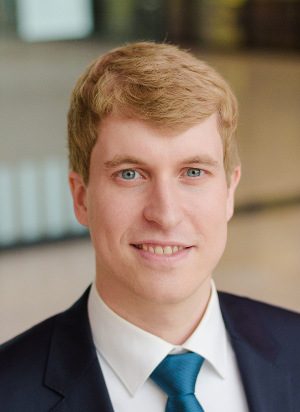
\includegraphics{Bewerbungsphoto_Edgar_300}
\section{geboren}
\color{gray}%
am 1986-08-13
in Pforzheim
\section{kontakt}
\color{gray}Dorfackerstra{\ss}e 19
72074 T\"ubingen
~
+49 175 3783003
~
\href{mailto:ed.klenske@gmx.de}{ed.klenske@gmx.de}
\section{fokus}
machine {\bfseries learning}
predictive {\bfseries control}
\section{sprachen}
{\bfseries deutsch} Muttersprache
{\bfseries englisch} fließend
~
{\bfseries Matlab} fließend 
{\bfseries C++} fortgeschritten
{\bfseries Python} Grundlagen
\end{aside}

%-------------------------------------------------------------------------------
% EDUCATION SECTION
%-------------------------------------------------------------------------------
\
\section{ausbildung}\normalfont

\begin{entrylist}
%------------------------------------------------
\entry
{2012-11 \to heute}
{Promotion {\normalfont in Machine Learning}}
{Max-Planck-Institut für Intelligente Systeme, T\"ubingen}
{\emph{Adaptive Autoguiding and Intelligent Control}.\\
Betreuer: Philipp Hennig, Bernhard Schölkopf, Melanie Zeilinger.}
%------------------------------------------------
\entry
{2006-10 \to 2012-07}
{Diplom {\normalfont in Technischer Kybernetik (Note 1,6)}}
{Universität Stuttgart, Germany}
{Diplomarbeit: \emph{Nonparametric System Identification and Control for
Periodic Error Correction in Telescopes} (Note: 1,0).\\
Betreuer: Philipp Hennig, Stefan Harmeling, Gregor G\"obel.
}
%------------------------------------------------
\entry
{1996-09 \to 2005-06}
{Abitur (Note: 1,3)}
{Theodor-Heuss-Gymnasium, Pforzheim}
{}
%------------------------------------------------
\end{entrylist}

%-------------------------------------------------------------------------------
% PUBLICATIONS SECTION
%-------------------------------------------------------------------------------

\section{publikationen}

{\Large \bfseries Artikel in Fachzeitschriften}

\bibentry{Dual Control for Approximate Bayesian Reinforcement Learning}{E.D.
Klenske, P. Hennig}{Journal of Machine Learning Research, \emph{accepted}.
\href{http://arxiv.org/abs/1510.03591}{\to arXiv}
}

\bibentry{Gaussian Process Based Predictive Control for Periodic
Error Correction}
{E.D. Klenske, M.N. Zeilinger, B. Sch\"olkopf, P. Hennig}
{IEEE Transactions on Control Systems Technology, 2016.
\href{http://dx.doi.org/10.1109/TCST.2015.2420629}{\to DOI},
\href{https://is.tue.mpg.de/uploads_file/attachment/attachment/9/%
Klenske_tcst__1_.pdf}{\to PDF}
}

{\Large \bfseries Artikel in Konferenzen}

\bibentry{Approximate Dual Control Maintaining the Value of Information
with an Application to Building Control}{E.D. Klenske, P. Hennig,
B. Sch\"olkopf, M.N. Zeilinger}{Proceedings of the European Control Conference,
2016.}

\bibentry{Nonparametric Dynamics Estimation for Time Periodic Systems}{E.D.
Klenske, M.N. Zeilinger, B. Sch\"olkopf, P. Hennig}{Proceedings of the 51st
Annual Allerton Conference on Communication, Control, and Computing, 2013.
\href{http://dx.doi.org/10.1109/Allerton.2013.6736564}{\to DOI}
}


% {\Large \bfseries theses}
%
% \bibentry{Nonparametric System Identification and Control for
% Periodic Error Correction in Telescopes}
% {E.D. Klenske}
% {Diplom thesis for the University of Stuttgart, 2012.
% \href{http://www.is.tuebingen.mpg.de/fileadmin/user_upload/files/publications/%
% 2012/Klenske_DiplomaThesis_01.pdf}{\to PDF}
% }

% \bibentry{Visualisierung linguistischer Merkmale (Visualization of Linguistic
% Features)}
% {E.D. Klenske}
% {Research thesis for the University of Stuttgart, 2011}

%-------------------------------------------------------------------------------
% WORK EXPERIENCE SECTION
%-------------------------------------------------------------------------------

\section{praktische erfahrung}

\begin{entrylist}
%------------------------------------------------
\entry
{2006-08 \to 2013-12}
{Eigentümer}
{Implexus Computerservice, Tiefenbronn}
{Computer-Service für kleine Unternehmen und Endkunden (Nebenerwerb)}
%------------------------------------------------
\entry
{2011-03 \to 2011-05}
{Internship}
{ESG Elektroniksystem- und Logistik GmbH, F\"urstenfeldbruck}
{Modellierung von Verkehrsregeln für Fahrerassistenzsysteme}
%------------------------------------------------
\end{entrylist}

%-------------------------------------------------------------------------------
% AWARDS SECTION
%-------------------------------------------------------------------------------

\section{preise \& auszeichnungen}\normalfont

\begin{entrylist}
%------------------------------------------------
\entry
{2010-12 \to 2013-04}
{VDI Elevate Stipendiat}
{Verein Deutscher Ingenieure}
{Stipendium mit Sozialkompetenz- und Management-Seminaren}
%------------------------------------------------
\entry
{2005-07}
{Ferry-Porsche-Preis}
{Dr. Ing. hc F. Porsche AG}
{für hervorragende Leistungen in Mathematik und Physik}
%------------------------------------------------
\end{entrylist}

\clearpage

\smallheader{Edgar}{Klenske}

%-------------------------------------------------------------------------------
% INVITED TALKS SECTION
%-------------------------------------------------------------------------------

\section{vorträge \& besuche} \bodyfont
\begin{itemize}
 \item Workshop on Analytic Probabilistic Radiation Treatment Planning, 
    Tübingen, 2016
 \item Institut für Technik Autonomer Systeme, Universität der Bundeswehr, 
    München, 2016
 \item Workshop on Learning Control, Tübingen, 2015
 \item Bosch Research, Renningen, 2015
 \item Computational Learning \& Motor Control Lab, University of Southern
    California, 2014
 \item EE \& CS Department, University of California at Berkeley, 2014
 \item Machine Learning and Robotics Colloquium, Universität Stuttgart, 2014
 \item Heidelberger Life-Science Lab, 2012
\end{itemize}


%-------------------------------------------------------------------------------
% COMMUNICATION SKILLS SECTION
%-------------------------------------------------------------------------------
{\raggedright
% \sloppy
\section{engagement} \bodyfont
{\Large \bfseries Summer Schools}
\begin{itemize}
 \item Machine Learning Summer School (MLSS), T\"ubingen, 2013 \& 2015: Leitung 
des Teams für Video- Aufzeichnungen und -Verarbeitung.
Verfügbar auf \href{
https://www.youtube.com/playlist?list=PLqJm7Rc5-EXFv6RXaPZzzlzo93Hl0v91E } {\to
youtube}
\end{itemize}

{\Large \bfseries Reviewer für}
\begin{itemize}
 \item Neural Information Processing Systems (NIPS)
 \item International Conference on Machine Learning (ICML)
 \item Journal for Machine Learning Research (JMLR)
\end{itemize}

{\Large \bfseries Lehrassistenz}
\begin{itemize}
 \item Assistent für die Vorlesung \emph{Intelligent Systems I} an der 
Universität T\"ubingen (WS 2012)
\item Assistent für die Vorlesung \emph{Echtzeitdatenverarbeitung} an der 
Universität Stuttgart (SS 2009)
\end{itemize}

% {\Large \bfseries Öffentlichkeitsarbeit}
% \begin{itemize}
%  \item Wochenendseminar zum Thema \emph{Wahrscheinlichkeit und Unsicherheit} 
% für hochbegabte Schüler, in Kollaboration mit dem Heidelberger Life Science 
% Lab, März 2013 
% %(mit Philipp Hennig und Martin Kiefel)
% \end{itemize}

{\Large \bfseries Ehrenamtliche Arbeit}
\begin{itemize}
 \item Doktorandensprecher der Abteilung \emph{Empirische Inferenz} am
Max-Planck-Institut für Intelligente Systeme, T\"ubingen (1~Jahr)
 \item Studentenvertreter in der Studienkommission Technische 
Kybernetik, Universität Stuttgart (2~Semester)
\item Studentenvertreter in der Berufungskommission \emph{Computation in
Control}, Universität Stuttgart
\item Studentenvertreter in der \emph{Gemeinsamen Kommission Maschinenbau},
Universität Stuttgart (2~Semester)
 \item Stellvertretender Vorsitzender des Studentenvereins für 
Netzwerksicherheit und Technologietransfer, \emph{WH-Netz e.V.} (1~Jahr)
\end{itemize}
}

% \section{referenzen} \bodyfont


\end{document}
